% \documentclass[../Main.tex]{subfiles}
% \externaldocument{0.0.overview}



% \begin{document}
\chapter{Distillation-Based Methods for Fast Sampling}\label{ch:distillation}

This chapter introduces training-based approaches that accelerate diffusion model sampling by teaching new generators to produce samples in only one or a few steps. The central idea, called \emph{distillation}, is to let a fast student model learn from a slow, pre-trained diffusion model (teacher) sampler. While the teacher may require hundreds of steps, the student can achieve comparable quality in only a few steps\footnote{Here, distillation refers to reducing the number of sampling steps, not to shrinking the model size.}. Unlike solver-based acceleration, which improves the numerical integration scheme, distillation directly trains a generator to take efficient shortcuts. We highlight two main paradigms: \emph{distribution level distillation}, which skips simulating the full trajectory and instead aligns the student’s output distribution with the teacher’s, and \emph{flow map level distillation}, which trains the student to reproduce the teacher’s sampling path in a faster and more compact way.

% This chapter introduces training-based methods for obtaining a one- or few-step denoiser (generator) for fast sampling by assuming an access to some well-trained pre-trained DM $\rvs_{\bm{\phi}^\times}(\rvx_s, s) \approx \nabla_{\rvx_s} \log p_s(\rvx_s)$. With the pre-trained DM, it can provides a proxy to $p_{\mathrm{data}}$ via sampling trajectory (i.e., SDE/ODE solving) as highlighted in \Cref{subsec:sde-sample}. the  The high-level idea of common approaches is either to distill the trajectory, or the learned distributions of a pre-trained diffusion model (teacher) into a fewer-steps generator from noise to a clean estimate.




% , which is supposed to be a proxy to $p_{\mathrm{data}}$ while sampling from its requires SDE/ODE solving as highlighted in \Cref{subsec:sde-sample}. Many approaches were proposed to extract either its sampling trajectory (we call it \emph{Trajectory Distillation}) into a few step generators or extract distribution modeled by the pre-trained DM (we refer to \emph{Distributional Distillation})
\clearpage
\newpage


\section{Prologue}\label{sec:distillation-prologue}
A central bottleneck of diffusion models is their slow sampling speed.  

As shown through Tweedie's formula (\Cref{subsec:four-equiv-para}), a diffusion model can be interpreted as an ``$\rvx$-prediction'' model, $\rvx_{\bm{\phi}^\times}(\rvx_t, t)$, trained to recover the expected clean data from a noisy input $\rvx_t$ at noise level $t$:
\[
    \rvx_{\bm{\phi}^\times}(\rvx_t, t) \approx \mathbb{E}[\rvx_0 |\rvx_t],
\]
where the expectation is taken with respect to $p(\rvx_0 |\rvx_t)$, representing all plausible clean data corresponding to $\rvx_t$.  
A natural idea is to use $\rvx_{\bm{\phi}^\times}(\rvx_t, t)$ for one step generation. Yet because this denoiser averages over many plausible outcomes, the prediction becomes overly smooth, and generation with only a few denoising steps leads to blurry, low quality samples.  

On the other hand, as discussed in \Cref{subsec:sde-sample}, diffusion sampling follows an ODE or SDE trajectory through a long sequence of iterative steps. This produces high fidelity samples, but the large number of steps required makes the process inherently slow. Reducing the NFE (i.e., the number of sampling steps times model calls) speeds up generation but inevitably reduces fidelity. 
Each solver step introduces an integration error of order $\mathcal{O}(h^{n})$, 
where $n$ is the solver order and $h=\max_i |t_i - t_{i-1}|$ is the step size.
Fewer steps imply a larger time increment $h$, which in turn increases the accumulated sampling error and leads to a less accurate trajectory.
 This creates a fundamental trade off between quality and efficiency in diffusion sampling.  

To overcome this bottleneck, a major line of research is \emph{distillation}, which assumes access to a well-trained diffusion model (the \emph{teacher}) and trains a generator (the \emph{student}) to reproduce its behavior through a single feed forward or few step computation. 
This compresses the teacher’s many sampling steps into a fast process, effectively bypassing slow iterative solvers while maintaining high sample fidelity.




Below, we introduce two perspectives on distillation: \emph{distribution level distillation} and \emph{flow map level distillation}\footnote{Chronologically, flow map level distillation, represented by \emph{Knowledge Distillation} (KD)~\citep{luhman2021knowledge} and \emph{Progressive Distillation} (PD)~\citep{ho2020denoising}, was proposed earlier in 2021, preceding the family of distribution level distillation approaches that emerged around 2023. For smoother exposition and connection to the next chapter, however, we present distribution level distillation first.}.





\subsection{Distribution Level Distillation}  
The goal of distribution-based distillation is to train a one-step generator $\rmG_{\bm{\theta}}(\rvz)$ that maps noise $\rvz \sim p_{\mathrm{prior}}$ to a sample $\hat\rvx = \rmG_{\bm{\theta}}(\rvz)$, inducing a distribution $p_{\bm{\theta}}(\hat\rvx)$ that approximates the target data distribution $p_{\mathrm{data}}(\rvx)$. This is typically achieved by minimizing a statistical divergence
\[
\min_{\bm{\theta}}  \mathcal{D}\!\left(p_{\bm{\theta}}(\hat\rvx),  p_{\mathrm{data}}(\hat\rvx)\right),
\]
where $\mathcal{D}$ denotes a suitable divergence measurement such as KL.  

In practice, distribution based methods align the generator’s distribution with the empirical distribution $p_{\bm{\phi}^\times}(\rvx)$ produced by a pre-trained diffusion model:
\[
\min_{\bm{\theta}}  \mathcal{D}\!\left(p_{\bm{\theta}}(\hat\rvx),  p_{\bm{\phi}^\times}(\hat\rvx)\right),
\]
where $p_{\bm{\phi}^\times}$ serves as a surrogate for $p_{\mathrm{data}}$. Rather than evaluating this divergence explicitly, these methods approximate its gradient, which can be computed directly from the pre-trained teacher model. 
This enables the student to align its distribution with the teacher’s without requiring full divergence evaluation.

This formulation distills multi-step generative processes of diffusion models into a single step model through distributional alignment. We detail this approach in \Cref{sec:VSD}.




\subsection{Flow Map Level Distillation} We consider the PF-ODE, which can be expressed for any prediction model (see \Cref{eq:predictions-equivalence}):
\begin{align}\label{eq:pf-ode-ct}
    \frac{\diff \rvx(\tau)}{\diff \tau} 
    = f(\tau) \rvx(\tau) - \tfrac{1}{2}g^2(\tau) \nabla_\rvx \log p_\tau(\rvx(\tau)) 
    =: \rvv^*(\rvx(\tau), \tau).
\end{align}

Its solution map, starting from $\rvx_s$ at time $s$ and evolving reversely to time $t \leq s$, is denoted by $\bPsi_{s\to t}(\rvx_s)$; that is,
\begin{align}\label{eq:int_target_gt}
\begin{aligned}
    \bPsi_{s\to t}(\rvx_s) 
    &\coloneqq \rvx_s + \int_s^t \rvv^*(\rvx(\tau), \tau) \diff \tau,
\end{aligned}
\end{align}
where the integral solves the PF-ODE. Intuitively, $\bPsi_{s\to t}$ transports, $\rvx_s$, noise at time $s$ to less noisy states at time $t$ (ultimately data at $t=0$).


Sampling from a diffusion model corresponds to evaluating $\bPsi_{T\to 0}(\rvx_T)$ for $\rvx_T \sim p_{\mathrm{prior}}$. Typically, this integral is approximated by iterative numerical solvers leveraging the velocity field $\rvv$ (see \Cref{ch:solvers}), but requires many steps (e.g., at least $10$ steps even in DPM-Solver), making sampling slower than classic one-step generative models such as GAN. This motivates a natural question:
\begin{question}
    Can we learn the solution map $\bPsi_{s\to t}(\rvx_s)$ directly? 
\end{question}
In particular, learning a map $\bPsi_{T\to 0}(\rvx_T)$ with $\rvx_T \sim p_{\mathrm{prior}}$ enables one-step generation.


\paragraph{Trajectory Distillation.}

Trajectory distillation seeks to train a neural generator that approximates the solution map at the instance level. Since the PF-ODE integral rarely admits a closed form, it must be approximated numerically during training. To formalize, we introduce the general solver notation
\begin{align}\label{eq:solver}
    \mathtt{Solver}_{s\to t}(\rvx_s;\,\bm{\phi}^\times)
    \quad \text{or simply} \quad
    \mathtt{Solver}_{s\to t}(\rvx_s),
\end{align}
denoting numerical integration of the empirical PF-ODE from $s$ to $t$ starting
at $\rvx_s$, with teacher parameters $\bm{\phi}^\times$ (omitted when clear from
context). 



\paragraph{An Early Approach: Direct Knowledge Distillation.}
To enable few step or even one step generation, a direct approach is to train a generator $\rmG_\btheta(\rvx_T, T,0)$ to imitate the output of a numerical solver evaluated along the full trajectory:
\[
\rmG_\btheta(\rvx_T, T,0)\approx \mathtt{Solver}_{T\to 0}(\rvx_T), 
\qquad \rvx_T \sim p_{\mathrm{prior}}.
\]
This idea underlies one of the earliest trajectory distillation methods, \emph{Knowledge Distillation}~\citep{luhman2021knowledge}, which uses the regression loss
\[
\mathcal{L}_{\mathrm{KD}}(\btheta)
:= 
\E_{\rvx_T \sim p_{\mathrm{prior}}}
\left\|
\rmG_\btheta(\rvx_T, T,0)
-
\mathtt{Solver}_{T\to 0}(\rvx_T)
\right\|_2^2.
\]
While this approach provides direct supervision from the pre-trained teacher,
it cannot leverage the strong supervision available in the original training data.
In addition, it is computationally expensive if ODE integration is invoked within
the training loop, since each parameter update requires solving the ODE to form
targets. Finally, because the generator learns only a global mapping from $T$ to $0$, it may lose controllability for steering the generation process from intermediate states. Consequently, most controllable generation techniques introduced in \Cref{ch:guidance} cannot be directly applied.




\paragraph{Preface to Progressive Distillation.}
\emph{Progressive Distillation} (PD)~\citep{salimans2021progressive} trains a time–conditional $ \mathtt{Student} $ using \emph{local} supervision from $\mathtt{Teacher}$ fragments. 
Let $t_0=T>t_1>\cdots>t_N=0$ be a fixed time grid. 
The $ \mathtt{Teacher} $ provides time–stepping maps $\mathtt{Teacher}_{t_k\to t_{k+1}}$ for $k=0,\ldots,N-1$.


Rather than supervising only the one-jump $T\to 0$, PD trains the $ \mathtt{Student}  $ two–step skip map to match two consecutive $ \mathtt{Teacher}$ steps:
\[
\mathtt{Student}_{t_k\to t_{k+2}}
\;\approx\;
\mathtt{Teacher}_{t_{k+1}\to t_{k+2}}
\circ
\mathtt{Teacher}_{t_{k}\to t_{k+1}},
\]
for $k = 0, 2, 4, \dots$.
The matching is performed using a simple regression loss (e.g., mean squared error).


After training on locally paired fragments, the $ \mathtt{Student} $ no longer follows every time interval of the original grid. 
Instead, it advances on every other time point,
\[
t_0 \to t_2 \to t_4 \to \cdots \to t_N,
\]
which means that each $ \mathtt{Student} $ step effectively covers two consecutive $ \mathtt{Teacher}$  steps. 
Consequently, the $ \mathtt{Student} $ completes the same overall time span $[0,T]$ using only $N/2$ transitions. 

After this stage, the trained $ \mathtt{Student} $ replaces the $ \mathtt{Teacher}$  to serve as the new reference model. 
The entire procedure is then repeated on the coarser grid, where the time step doubles 
$(N \to N/2 \to N/4 \to \cdots)$,
progressively distilling the trajectory into fewer and fewer steps until the desired number of inference steps is reached. 
This iterative halving preserves the global time horizon while continually compressing the temporal resolution of the generative process.






\paragraph{A Unified Perspective of Flow Map Learning.}
Various methods, including KD and PD, can be expressed within a unified loss framework:
\begin{align}\label{eq:general-cm-loss}
  \mathcal{L}_{\mathrm{oracle}}(\btheta)
  := \E_{s,t} \E_{\rvx_s \sim p_s} 
  \left[  w(s,t)  d \big(\rmG_\btheta(\rvx_s, s,t),  \bPsi_{s\to t}(\rvx_s)\big)\right],
\end{align}
where $\bPsi_{s\to t}$ is the oracle flow map, $w(s,t) \geq 0$ specifies how different time pairs $(s,t)$ are weighted,
$d(\cdot,\cdot)$ is a discrepancy measure such as
$d(\rvx,\rvy)=\|\rvx-\rvy\|_2^2$ or $d(\rvx,\rvy)=\|\rvx-\rvy\|_1$,  and $p_s$ denotes the
forward noised marginal at time $s$. Because $\bPsi_{s\to t}$ is not available
in closed form, one must rely on approximations, typically through a pre-trained
diffusion model (teacher) or another tractable surrogate.

KD appears as a simple instance of
\Cref{eq:general-cm-loss}. Selecting a degenerate weighting
$w(s,t)=\delta(s{-}T)\,\delta(t{-}0)$ and using the prior distribution
$p_T=p_{\mathrm{prior}}$\footnote{This assumption holds for large enough $T$ or
with appropriate noise schedules $(\alpha_t,\sigma_t)$.}, the oracle loss $\mathcal{L}_{\mathrm{oracle}}(\btheta)$ reduces to:
\[
\E_{\rvx_T\sim p_T}
\big\|\rmG_\btheta(\rvx_T,T,0)-\bPsi_{T\to 0}(\rvx_T)\big\|_2^2
\approx \mathcal{L}_{\mathrm{KD}}(\btheta),
\quad
\]
with $\mathtt{Solver}_{T\to 0}\approx\bPsi_{T\to 0}$. An alternative perspective on this formulation is presented in \Cref{app-sec:flow-map}.


PD also fits this template, but instead of supervising only with the single extreme pair $(T,0)$, it uses many \emph{nearby} time pairs and enforces a simple \emph{local consistency} rule:
a short step followed by another short step should match the direct two–step move. We return to this in \Cref{eq:pd-local}.

In practice, the main challenge is that the oracle flow map $\bPsi_{s\to t}$ generally has no closed-form expression, making direct supervision infeasible.  A range of methods have been developed to approximate this
target efficiently, but their success often hinges on the quality of the teacher
model. We will return to \Cref{eq:general-cm-loss} in \Cref{ch:fast-scratch}, presenting a principled framework for training-from-scratch methods that eliminate the teacher from the learning loop.








\clearpage
\newpage



\section{\texorpdfstring{Distribution-Based Distillation}{Distribution-Based Distillation}}\label{sec:VSD}


Several works have pursued this distribution-based distillation concurrently under different names,
including Distributional Matching Distillation (DMD)~\citep{yin2024one,yin2024improved},
Variational Score Distillation (VSD)~\citep{pooledreamfusion,wang2023prolificdreamer,luo2023diff,lu2024simplifying},
and Score Identity Distillation (SiD)~\citep{zhou2024score}.
Despite technical differences, they share the same principle:
train a generator whose forward-noised marginals match those of the teacher.
We focus on VSD as a representative formulation, since the others follow similar principles.


\subsection{Formulation of VSD as a Representative Approach}
\paragraph{Forward Process.}
Let $\{p_t\}_{t \in [0,T]}$ denote the marginal densities of a forward diffusion process induced by
\[
\rvx_t = \alpha_t \rvx_0 + \sigma_t \bm{\epsilon}, \quad \bm{\epsilon} \sim \mathcal{N}(\bm{0}, \rmI),
\]
with initial distribution $p_0 = p_{\mathrm{data}}$.  
In contrast, let $p_0^{\bm{\theta}}$ denote the distribution of synthetic samples generated by a deterministic one-step generator $\rmG_{\bm{\theta}}(\rvz)$ from latent variables $\rvz \sim p_{\mathrm{prior}}(\rvz)$. Define $\{p_t^{\bm{\theta}}\}_{t \in [0,T]}$ as the marginal densities obtained by applying the same forward diffusion process to $p_0^{\bm{\theta}}$, that is,
\begin{align}\label{eq:vsd-forward}
    \rvx_t^{\bm{\theta}} := \alpha_t \rmG_{\bm{\theta}}(\rvz) + \sigma_t \bm{\epsilon}, 
\end{align}
where $\rvz \sim p_{\mathrm{prior}}$ and $ \bm{\epsilon} \sim \mathcal{N}(\bm{0}, \rmI)$. Thus, both $p_t$ and $p_t^{\bm{\theta}}$ share the same Gaussian diffusion kernel 
$p_t(\rvx_t| \rvx_0)$ but differ in their starting distributions 
($p_{\mathrm{data}}$ vs.\ $p_0^{\bm{\theta}}$ of one-step synthetic samples).

\paragraph{Training Objective and Gradient.}
The literature typically adopts the KL divergence to match the distributions $p_t$ and $p_t^{\bm{\theta}}$, commonly by minimizing
\begin{align*}
    \mathcal{L}_{\text{VSD}}(\bm{\theta}) &:=\mathbb{E}_t \left[ \omega(t)  \mathcal{D}_{\text{KL}}(p_t^{\bm{\theta}} \, \| \, p_t) \right]
\\&= \mathbb{E}_{t, \rvz, \bm{\epsilon}} \left[ \omega(t) \left( \log p_t^{\bm{\theta}}(\rvx_t^{\bm{\theta}}) - \log p_t(\rvx_t^{\bm{\theta}}) \right) \right],
\end{align*}
where $\omega(t)$ is a time-dependent weighting function. We will discuss in \Cref{subsec:vsd-discussion} why the KL divergence plays a
special role in distribution-level distillation.



As shown in \citep{wang2023prolificdreamer}, the optimum is achieved when $ p_0^{\bm{\theta}^*} = p_{\mathrm{data}} $, indicating that the generator's distribution matches the data distribution, and the training objective serves as a valid loss for learning the data distribution.

However, the density-based formulation of the objective lacks an efficient training mechanism. Fortunately, by taking the gradient with respect to $\bm{\theta}$, we arrive at the expression in \Cref{eq:vsd-grad}, which is summarized in the following proposition. For notational simplicity, we denote $\hat\rvx_t := \rvx_t^{\bm{\theta}}$ as defined in \Cref{eq:vsd-forward}.




\proppp{$\bm{\theta}$-Gradient of $\mathcal{L}_{\text{VSD}}$}{vsd-grad}{
We have
\begin{align}\label{eq:vsd-grad}
\begin{aligned}
        &\nabla_{\bm{\theta}}\mathcal{L}_{\text{VSD}}(\bm{\theta}) \\= &\mathbb{E}_{t, \rvz, \bm{\epsilon}} \left[ \omega(t)\alpha_t  \left( 
\nabla_{\rvx} \log p_t^{\bm{\theta}}(\hat\rvx_t) - \nabla_{\rvx} \log p_t(\hat\rvx_t) 
\right) \cdot \partial_{\bm{\theta}} \rmG_{\bm{\theta}}(\rvz) \right].
\end{aligned}
\end{align}
}{
The derivation applies the chain rule:
\begin{align*}
&\nabla_{\btheta} \E_t \left[ \mathcal{D}_{\mathrm{KL}}(p_t^{\btheta}\|p_t) \right]
\\&= \E_{t,\rvz,\beps}\!\left[\partial_\btheta
\big(\log p_t^{\btheta}(\hat\rvx_t)-\log p_t(\hat\rvx_t)\big) \right] \\
&= \E_{t,\rvz,\beps} \left[ 
 \underbrace{\partial_{\btheta}\log p_t^{\btheta}(\hat\rvx_t)}_{\text{first}}
+ (\nabla_{\rvx}\log p_t^{\btheta}(\hat\rvx_t))^\top \partial_{\btheta}\hat\rvx_t
- (\nabla_{\rvx}\log p_t(\hat\rvx_t))^\top \partial_{\btheta}\hat\rvx_t \right].
\end{align*}
The first term vanishes by the score-function identity:
\[
\E_{\hat\rvx_t\sim p_t^{\btheta}}\!\left[\partial_{\btheta}\log p_t^{\btheta}(\hat\rvx_t)\right]
= \int \partial_{\btheta} p_t^{\btheta}(\rvx)  \diff\rvx
= \partial_{\btheta}  \int p_t^{\btheta}(\rvx)  \diff\rvx
= \partial_{\btheta}(1)=0.
\]
Using the reparameterization $\hat\rvx_t=\alpha_t\rmG_{\btheta}(\rvz)+\sigma_t\beps$ gives
$\partial_{\btheta}\hat\rvx_t=\alpha_t\partial_{\btheta}\rmG_{\btheta}(\rvz)$, hence
\[
\nabla_{\btheta}\mathcal{L}_{\text{VSD}}(\btheta)
= \E_{t,\rvz,\beps} \left[\omega(t) \alpha_t 
\big(\nabla_{\rvx}\log p_t^{\btheta}(\hat\rvx_t)-\nabla_{\rvx}\log p_t(\hat\rvx_t)\big)^\top
\partial_{\btheta}\rmG_{\btheta}(\rvz)\right].
\]
This proves \Cref{eq:vsd-grad}.
See \Cref{app-sec:flow-map} for details.
}


We observe that the score functions naturally emerge when taking the gradient
with respect to $\bm{\theta}$. Consequently, we require approximations of
the score $\nabla_{\rvx}\log p_t^{\bm{\theta}}(\hat\rvx_t)$ for the
one-step generator and $\nabla_{\rvx}\log p_t(\hat\rvx_t)$ for the data
distribution, as will be detailed in the following subsection.








\subsection{Training Pipeline of VSD}\label{subsec:vsd-training}
Existing works~\citep{yin2024one,yin2024improved,pooledreamfusion,wang2023prolificdreamer,luo2023diff,lu2024simplifying} typically address this via a bi-level optimization approach: training a new diffusion model on samples from $\rmG_{\bm{\theta}}(\rvz)$ to approximate $\nabla_{\rvx} \log p_t^{\bm{\theta}}(\hat\rvx_t)$, and employing a pre-trained diffusion model to provide a proxy for the intractable oracle score function $\nabla_{\rvx} \log p_t(\hat\rvx_t)$ on synthetic samples $\hat\rvx_t$. More precisely, training proceeds by alternating between two phases:
\begin{itemize}
    \item \textbfs{Score Estimation Phase.} Fix $\bm{\theta}$. Let $\hat{\rvx}_0=\rmG_{\bm{\theta}}(\rvz)$ and
    $\hat{\rvx}_t=\alpha_t \hat{\rvx}_0+\sigma_t\beps$ with $\rvz\sim p_{\mathrm{prior}}$, $\beps\sim\mathcal{N}(\bm{0},\rmI)$.
    Train $s_{\bm{\zeta}}$ by DSM using the known Gaussian diffusion kernel $p_t(\rvx_t|\rvx_0)$:
    \[
    \mathcal{L}_{\text{DSM}}(\bm{\zeta};\bm{\theta})
    =\E_{t,\rvz,\beps}\Big\|\,\rvs_{\bm{\zeta}}(\hat{\rvx}_t,t)
    - \nabla_{\rvx_t}\log p_t(\hat{\rvx}_t|\hat{\rvx}_0)\,\Big\|^2,
    \]
    which yields $\rvs_{\bm{\zeta}}(\cdot,t)\approx \nabla_{\rvx}\log p_t^{\bm{\theta}}(\cdot)$ at optimum (for fixed $\bm{\theta}$).
    

  \item \textbfs{Generator Update Phase.} With $s_{\bm{\zeta}}$ frozen (stop-grad),  $\bm{\theta}$ is updated by using the gradient in \Cref{eq:vsd-grad}, replacing the individual score terms by their respective proxies:
  \[
    \rvs_{\bm{\zeta}}(\hat\rvx_t,t)\approx \nabla_{\rvx}\log p_t^{\bm{\theta}}(\hat\rvx_t), \,\, \text{and} \,\, \rvs_{\bm{\phi}^\times}(\hat{\rvx}_t,t)\approx \nabla_{\rvx}\log p_t(\hat\rvx_t)\ \ \text{(teacher)}.
  \]
  \Cref{eq:vsd-grad} then approximately becomes:
  \[
    \nabla_{\bm{\theta}}\mathcal{L}_{\text{VSD}}(\bm{\theta})
    \approx \mathbb{E}_{t,\rvz,\bm{\epsilon}}\Big[\omega(t)\alpha_t
      \big(\rvs_{\bm{\zeta}}(\hat{\rvx}_t,t) - \rvs_{\bm{\phi}^\times}(\hat{\rvx}_t,t)\big)^{\top}
      \partial_{\bm{\theta}}\rmG_{\bm{\theta}}(\rvz)
    \Big].
  \]
\end{itemize}
These two phases repeat until, for all $t$, 
$\rvs_{\bm{\zeta}}(\cdot,t)\approx \rvs_{\bm{\phi}^\times}(\cdot,t)$ on the support of $p_t^{\bm{\theta}}$,
so the plug-in gradient in \Cref{eq:vsd-grad} vanishes. In this convergence regime,
we have $p_t^{\bm{\theta}}\approx p_t^{\bm{\phi}^\times}$ (the teacher’s marginal) for all $t>0$.
Since the forward noising operator (Gaussian convolution) is injective for any fixed $t>0$,
it follows that $p_0^{\bm{\theta}}\approx p_0^{\bm{\phi}^\times}$ (the teacher’s $t=0$ distribution).
Thus, the learned one-step generator $\rmG_{\bm{\theta}}$ matches the teacher’s distribution at $t=0$;
when the teacher closely approximates $p_{\mathrm{data}}$, this further implies $p_0^{\bm{\theta}}\approx p_{\mathrm{data}}$.

\subsection{Additional Discussion: Divergence Choices and VSD Applications}\label{subsec:vsd-discussion}


\paragraph{Beyond KL: Can We Use General Divergences?}
In principle, one may replace the forward KL term
$\mathcal{D}_{\mathrm{KL}}(p_t^{\btheta}\|p_t)$ in VSD with a more general
divergence family, such as the  $f$-divergence (see \Cref{eq:f-div}):
\[
\mathcal{D}_f(p_t^{\btheta}\|p_t)
= \int p_t(\rvx)  f\!\left(\frac{p_t^{\btheta}(\rvx)}{p_t(\rvx)}\right)\diff \rvx.
\]
However, the gradient
$\nabla_{\btheta}\mathcal{D}_f(p_t^{\btheta}\|p_t)$ depends on the
\emph{density ratio}
\[
r_t(\rvx)=\frac{p_t^{\btheta}(\rvx)}{p_t(\rvx)},
\]
through $f'(r_t)$, which is intractable for an \emph{implicit student generator}.
Here the student is called \emph{implicit} because it can produce samples
$\hat\rvx_t$ through a stochastic mapping
$\hat\rvx_t=\alpha_t\rmG_\btheta(\rvz)+\sigma_t\beps$, but it does not provide
a closed-form expression or likelihood for its induced density
$p_t^{\btheta}(\rvx)$.
Consequently, computing the functional derivative of $\mathcal{D}_f$
requires pointwise access to $r_t(\rvx)$ or its log-gradient, both of which
cannot be evaluated in this setting.
A common workaround is to introduce an auxiliary critic or discriminator that
approximates the density ratio via the variational formulation of
$f$-divergences, as in $f$-GAN~\citep{nowozin2016f}, although this introduces an
extra network and a nested minimax optimization.

By contrast, for the forward KL, the pathwise gradient simplifies neatly to a score-difference form (\Cref{eq:vsd-grad}):
\[
\nabla_{\btheta}\mathcal{D}_{\mathrm{KL}}(p_t^{\btheta}\|p_t)
= \E\!\left[
  \big(\nabla_{\rvx}\log p_t^{\btheta}(\hat\rvx_t)
  - \nabla_{\rvx}\log p_t(\hat\rvx_t)\big)^\top
  \partial_{\btheta}\hat\rvx_t
\right].
\]
This structure enables a tractable score-only update. The teacher’s
pre-trained diffusion model already provides $\nabla_{\rvx}\log p_t(\cdot)$,
so we can reuse it directly without learning an auxiliary density-ratio
estimator. This formulation yields a non-adversarial training objective that remains fully
differentiable and computationally efficient.

\paragraph{VSD for 3D Generation Using Only a 2D pre-trained Diffusion Model.}
VSD~\citep{wang2023prolificdreamer}, together with its earlier special case SDS~\citep{pooledreamfusion} where the generator is a Dirac parameterized by $\btheta$, was originally introduced for 3D scenarios without paired supervision between 3D and 2D data (that is, without ground-truth 3D labels). 
Let $\btheta\in\R^d$ denote the parameters of a 3D scene, and let $\rmR(\btheta)$ be a differentiable renderer that produces an image $\hat{\rvx}_0:=\rmR(\btheta)$. 
The forward noising process is defined as
\[
\hat{\rvx}_t=\alpha_t\,\rmR(\btheta)+\sigma_t\beps,\quad \beps\sim\mathcal N(\bm 0,\rmI).
\]
A pre-trained 2D (image) diffusion teacher provides scores
\[
\rvs_{\bphi^\times}(\hat{\rvx}_t,t|\rvc)\approx\nabla_{\hat{\rvx}_t}\log p_t(\hat{\rvx}_t|\rvc),
\]
optionally conditioned on text $\rvc$. 
The goal is to align the distribution of noisy renderings with the teacher’s marginals at each $t$. 
A minimal formulation is the score-alignment (VSD) objective under the rendering distribution:
\[
\mathcal{L}^{\text{3D}}_{\text{VSD}}(\btheta)
:=\E_{t,\beps}\!\left[\omega(t)\,\big\|
\rvs_{\bm{\zeta}}(\hat{\rvx}_t,t)-\rvs_{\bphi^\times}(\hat{\rvx}_t,t|\rvc)
\big\|_2^2\right],
\quad \hat{\rvx}_t=\alpha_t\rmR(\btheta)+\sigma_t\beps,
\]
which transfers image-space score guidance to the 3D parameters through the renderer. 
Treating both scores as stop gradients with respect to $\hat{\rvx}_t$ during the update of $\btheta$ yields
\[
\nabla_{\btheta}\mathcal{L}^{\text{3D}}_{\text{VSD}}(\btheta)
=\E_{t,\beps}\!\left[\omega(t)\,\alpha_t\,
\big(\rvs_{\bm{\zeta}}-\rvs_{\bphi^\times}\big)^\top
\frac{\partial \rmR}{\partial\btheta}(\btheta)\right].
\]
When the student score $\rvs_{\bm{\zeta}}$ is suppressed (Dirac generator), the formulation reduces to SDS~\citep{pooledreamfusion}. 
In practice, optimization alternates exactly as described in \Cref{subsec:vsd-training}: first updating the student score on noisy renderings, and then updating $\btheta$ with stop gradients through both scores. 
Further mathematical details are omitted here for brevity.




\clearpage
\newpage

\section{\texorpdfstring{Progressive Distillation}{Progressive Distillation}}\label{sec:PD}


Progressive Distillation (PD)~\citep{salimans2021progressive} consists of two procedures that together enable a diffusion model to learn the PF-ODE trajectory more efficiently. 
The key idea is to progressively reduce the number of integration steps required for high-quality sampling while retaining fidelity to the teacher trajectory.
\begin{itemize}
    \item \textbfs{Distillation Operation:} Distills a deterministic sampler (e.g., DDIM) based on a pre-trained teacher model (initially a diffusion model) into a student model that reproduces the same trajectory using only half as many sampling steps.
    \item \textbfs{Progressive Operation:} Repeats this distillation process iteratively, each time halving the number of steps, until the student can generate high-quality samples within a small fixed budget (typically $1$–$4$ steps).
\end{itemize}

\begin{figure}[th!]
    \centering
    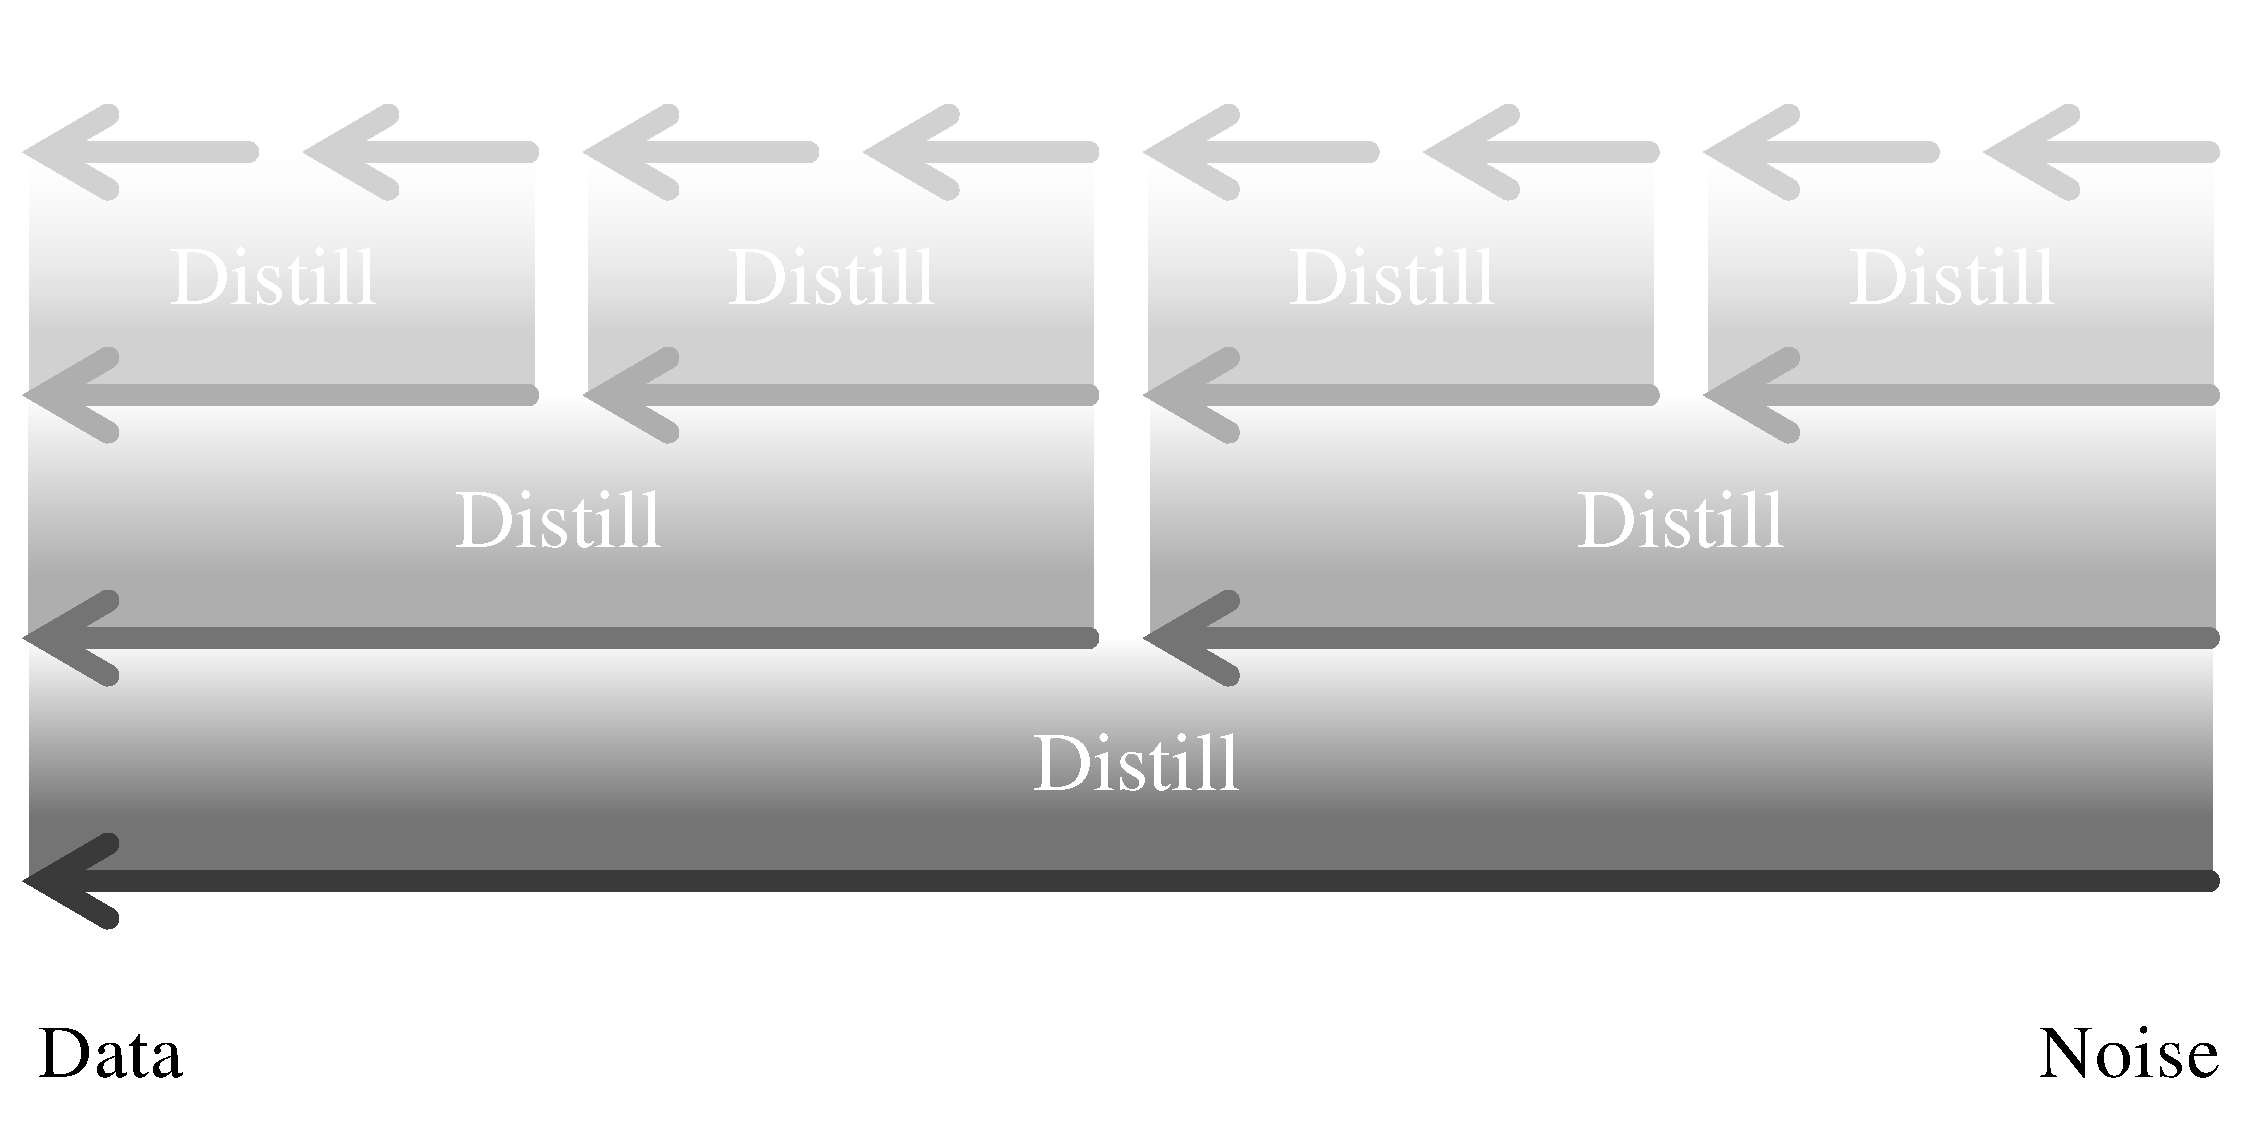
\includegraphics[width=0.93\linewidth]{Images/PartD/PD.pdf} 
    \caption{\textbfs{Illustration of Progressive Distillation (PD).} 
At each round, the student model is trained so that a single step reproduces the effect of two adjacent teacher steps. 
This process distills $N$ teacher steps into $N/2$ student steps, and repeating the procedure progressively halves the trajectory length until the desired step count is reached. 
The arrows indicate how multi-step teacher transitions are compressed into fewer student steps, moving from data to noise.
\figcredit{Created by the authors.}
}
    \label{fig:pd-illustration}
\end{figure}



We first introduce the distillation operation of PD in \Cref{subsec:pd-distillation}, and then summarize the entire training pipeline in \Cref{subsec:pd-training}. \Cref{subsec:pd-guidance} presents an extension for CFG guidance.


\subsection{Distillation Operation in PD}\label{subsec:pd-distillation}

In this section, we fix DDIM in the $\rvx$-prediction parameterization as the time–stepping rule and still write $\mathtt{Solver}_{s \to t}$ for the deterministic map obtained by plugging the current teacher’s $\rvx$-denoiser into DDIM.


In the first PD round (teacher = pre–trained diffusion model), this coincides with integrating the diffusion PF–ODE via DDIM; in later rounds (teacher = previous student), $\mathtt{Solver}_{s \to t}$ is simply the DDIM transition induced by the current teacher, not the original diffusion PF–ODE.


The distillation step is as follows: starting from a noisy input $\rvx_s$ (a perturbed version of clean data, $\rvx_s = \alpha_s \rvx_0 + \sigma_s \bm{\epsilon}$), the student is trained to predict a target ${\color{orange}\tilde\rvx}$ so that a single student step $s\!\to\! t$ reproduces the teacher’s two consecutive steps $s\!\to\! u\!\to\! t$.
Let $\rvx_{\bm{\phi}^\times}(\rvx,\tau)$ denote the teacher’s $\rvx$-prediction denoiser in this round.
Applying the teacher–induced DDIM transition twice gives
\[
\tilde\rvx_u := \mathtt{Solver}_{s\to u}\!\left(\rvx_s;\,\rvx_{\bm{\phi}^\times}\right),
\qquad
\tilde\rvx_t := \mathtt{Solver}_{u\to t}\!\left(\tilde\rvx_u;\,\rvx_{\bm{\phi}^\times}\right).
\]
Here, we use the notation of \Cref{eq:solver} to denote the deterministic transition map from $s$ to $t$ (starting at $\rvx_s$) induced by plugging $\rvx_{\bm{\phi}^\times}$ into DDIM.

\begin{question}
What is the pseudo-clean ${\color{orange}\tilde\rvx}$ at time $s$ such that the solver produces the same output $\tilde\rvx_t$ when stepping directly $s \to t$ as it does via $s \to u \to t$? Specifically, determine ${\color{orange}\tilde\rvx}$ satisfying:
\[
\tilde\rvx_t = \mathtt{Solver}_{s\to t}\left(\rvx_s; {\color{orange}\tilde\rvx}\right).
\]
\end{question}





Once a closed-form expression for ${\color{orange}\tilde\rvx}$ is obtained, we train a student model $\rvf_{\bm{\theta}}(\rvx_s, s)$ (also an $\rvx$-prediction model here) to approximate the ``two-steps-in-one'' target ${\color{orange}\tilde\rvx}$ by minimizing
\begin{align}\label{eq:pd-optimization}
\min_{\bm{\theta}} \E_s
\mathbb{E}_{\rvx_s\sim p_s}\!\left[w(\lambda_s)\,\big\|\rvf_{\bm{\theta}}(\rvx_s, s) - {\color{orange}\tilde\rvx}\big\|_2^2\right].
\end{align}


In the following, we show that the DDIM rule yields ${\color{orange}\tilde\rvx}$ in closed form through elementary algebra (note that the result holds for both discrete and continuous time):
\lemp{Two-Steps-in-One Target ${\color{orange}\tilde\rvx}$ of DDIM}{pd-ddim}{Starting from an initial condition $\rvx_s$, if the solver is taken as DDIM, then the ``two-step-in-one'' target ${\color{orange}\tilde\rvx}$ can be computed as
\begin{align*}
    {\color{orange}\tilde\rvx} 
    &=\frac{\sigma_s}{\alpha_t\sigma_s - \alpha_s\sigma_t} \tilde\rvx_t - \frac{\sigma_t}{\alpha_t\sigma_s - \alpha_s\sigma_t} \rvx_s.
\end{align*}
Here, $\tilde\rvx_t$ is obtained by applying DDIM (in \Cref{eq:ddim-update-all}) twice, from $s \to u \to t$:
\begin{align*}
    s \to u: & \quad    && \tilde\rvx_u = \frac{\sigma_u}{\sigma_s}\rvx_s + \alpha_s \left(\frac{\alpha_u}{\alpha_s} - \frac{\sigma_u}{\sigma_s} \right)\rvx_{\bm{\phi}^\times}(\rvx_s, s)  \\
    u \to t: & \quad    && \tilde\rvx_t = \frac{\sigma_t}{\sigma_u}\tilde\rvx_u + \alpha_u \left(\frac{\alpha_t}{\alpha_u} - \frac{\sigma_t}{\sigma_u} \right)\rvx_{\bm{\phi}^\times}(\tilde\rvx_u, u).
\end{align*}
}{$\tilde\rvx_t$ must be matched with the one-step DDIM from $s$ to $t$, $\tilde\rvx_t'$, expressed as:
\[
s \to t: \quad \tilde\rvx_t' = \frac{\sigma_t}{\sigma_s}\rvx_s + \alpha_s \left(\frac{\alpha_t}{\alpha_s} - \frac{\sigma_t}{\sigma_s} \right) {\color{orange}\tilde\rvx}.
\]
By equating $\tilde\rvx_t'$ and $\tilde\rvx_t$, we can solve for ${\color{orange}\tilde\rvx}$ in terms of $\tilde\rvx_t$, $s$, and $t$:
\begin{align}
    &\tilde\rvx_t = \tilde\rvx_t' \nonumber \\
    \Longleftrightarrow\,\, & \tilde\rvx_t = \frac{\sigma_t}{\sigma_s}\rvx_s + \alpha_s \left(\frac{\alpha_t}{\alpha_s} - \frac{\sigma_t}{\sigma_s} \right) {\color{orange}\tilde\rvx} \nonumber \\
    \Longleftrightarrow\,\, & {\color{orange}\tilde\rvx} =  \frac{\tilde\rvx_t - \frac{\sigma_t}{\sigma_s}\rvx_s}{\alpha_s \left(\frac{\alpha_t}{\alpha_s} - \frac{\sigma_t}{\sigma_s} \right)} \label{eq:x-pd-paper} \\
    \Longleftrightarrow\,\, & {\color{orange}\tilde\rvx} = \frac{\sigma_s}{\alpha_t\sigma_s - \alpha_s\sigma_t} \tilde\rvx_t - \frac{\sigma_t}{\alpha_t\sigma_s - \alpha_s\sigma_t} \rvx_s. \nonumber
\end{align}
}
With this formula, PD computes the pseudo-clean target at time $s$ whose single DDIM step $s\!\to\!t$ lands exactly at the two-step output $\tilde\rvx_t$.


\paragraph{Practical Discrete Time Grids and Loss.}
In practice, we fix a decreasing grid $t_0=T>t_1>\cdots>t_N=0$ and, for brevity, write $s:=t_k$, $u:=t_{k+1}$, $t:=t_{k+2}$.
The teacher provides one step maps $\mathtt{Teacher}_{t_k\to t_{k+1}}$, and the student learns a two step skip map that matches the teacher composition:
\[
\mathtt{Student}_{t_k\to t_{k+2}}
 \approx 
\mathtt{Teacher}_{t_{k+1}\to t_{k+2}}
\circ
\mathtt{Teacher}_{t_{k}\to t_{k+1}}.
\]

We sample triplets $(s,u,t)=(t_k,t_{k+1},t_{k+2})$ with $k\in\{0,\ldots,N-2\}$.
The objective \Cref{eq:pd-optimization} becomes
\[
\min_{\bm{\theta}} 
\mathbb{E}_{\,k \sim \mathcal{U}[\![0,N{-}2]\!]}\,
\mathbb{E}_{\,\rvx_{t_k}\sim p_{t_k}}\!
\Big[
  w(\lambda_{t_k})\,
  \big\|
  \rvf_{\bm{\theta}}(\rvx_{t_k},t_k) - {\color{orange}\tilde\rvx}^{(k)}
  \big\|_2^2
\Big],
\]
where the teacher two-step target ${\color{orange}\tilde\rvx}^{(k)}$ is computed via Lemma~\ref{pd-ddim}.  If the grid is uniform, one may write $t_k = T(1 - k/N)$ so that
\[
s = T\Big(1 - \frac{k}{N}\Big),\quad
u = T\Big(1 - \frac{k+1}{N}\Big),\quad
t = T\Big(1 - \frac{k+2}{N}\Big),
\]
corresponding to evenly spaced time steps of size $\Delta s =  T/N$.


\subsection{Entire Training Pipeline of PD and Its Sampling}\label{subsec:pd-training}
After training on locally paired fragments via \Cref{eq:pd-optimization}, the $\mathtt{Student}$ no longer follows every interval of the original grid. Instead, each learned step covers two consecutive $\mathtt{Teacher}$ steps, so the $\mathtt{Student}$ advances on every other time point,
\[
t_0 \to t_2 \to t_4 \to \cdots \to t_N,
\]
and thus traverses the same horizon $[0,T]$ using only $N/2$ transitions. After this stage, the trained $\mathtt{Student}$ replaces the $\mathtt{Teacher}$ as the new denoiser model. The procedure is then repeated on the coarser grid (the time step doubles), yielding the progression
\[
N \;\to\; N/2 \;\to\; N/4 \;\to\; \cdots,
\]
until the desired number of inference steps is reached. At each iteration, the new $\mathtt{Student}$ is initialized from the updated $\mathtt{Teacher}$. This iterative halving preserves the global time horizon while progressively compressing the temporal resolution of the generative process.

\paragraph{Sampling.}
At inference time, using the (DDIM) solver with the current $\mathtt{Student}$ as the denoiser, the sampler advances on the coarser grid induced by training. After the first round it takes ``skip-2'' jumps ($t_0 \to t_2 \to \cdots \to t_N$), after the next round ``skip-4'' ($t_0 \to t_4 \to \cdots \to t_N$), and so on, halving the number of sampling steps at each iteration while keeping the same start and end times.

\subsection{Additional Discussion: Local Semigroup Matching and the Possibility of Generalized Solvers}


\paragraph{Progressive Distillation as Local Semigroup Matching.}
Within the unified objective \Cref{eq:general-cm-loss}, the intractable oracle
target $\bPsi_{s\to 0}$ is replaced by a teacher–induced surrogate that uses the
\emph{semigroup property} of the ODE flow (see more details later in \Cref{eq:semi-group}): evolving from $s$ to $t$ should be
equivalent to going from $s$ to any intermediate $u$ and then from $u$ to $t$,
\[
\bPsi_{s\to t} = \bPsi_{u\to t}\circ\bPsi_{s\to u}.
\]
PD enforces this locally by training the student’s one–step map to match the
teacher’s composition of two adjacent one–step fragments:
\begin{align}\label{eq:pd-local}
  \E_{s}\E_{\rvx_s\sim p_s}
  \big\|
    \underbrace{\rmG_{\btheta}(\rvx_s, s, s-2\Delta s)}_{\text{student one-step}}
    -
    \underbrace{\mathtt{Solver}_{s-\Delta s\to s-2\Delta s}\big(\mathtt{Solver}_{s\to s-\Delta s}(\rvx_s)\big)}_{\text{teacher two-step composition}}
  \big\|_2^2.
\end{align}
Minimizing \Cref{eq:pd-local} instantiates the semigroup identity on a short
decreasing grid (take $s>u>t$ with $u=s-\Delta s$ and $t=s-2\Delta s$):
\begin{align*}
  \bPsi_{s\to s-2\Delta s}
  &= \bPsi_{s-\Delta s\to s-2\Delta s}\circ\bPsi_{s\to s-\Delta s}
  \\&\approx
  \mathtt{Solver}_{s-\Delta s\to s-2\Delta s}\circ \mathtt{Solver}_{s\to s-\Delta s},
\end{align*}
so training only requires short teacher fragments, rather than a full rollout
from time $s$ all the way to $0$.

To connect back to the few–step denoiser view in \Cref{eq:general-cm-loss}, define
the student’s few–step map as a composition of learned jumps:
\[
\underbrace{\rmG_{\btheta}(\rvx_s, s, 0)}_{\text{few-step denoiser}}
=
\big(\rmG_{\btheta}(\,\cdot\,, 2\Delta s, 0)\circ\cdots\circ \rmG_{\btheta}(\,\cdot\,, s, s-2\Delta s)\big)(\rvx_s).
\]
Conceptually, \Cref{eq:pd-local} provides an efficient \emph{local surrogate} for the
global regression
\[
\E_{s,\rvx_s}\Big\|\rmG_{\btheta}(\rvx_s,s,0)\;-\;(\mathtt{Solver})^{\circ}_{s\to 0}(\rvx_s)\Big\|_2^2,
\]
where $(\mathtt{Solver})^{\circ}_{s\to 0}$ denotes the teacher’s full
composition from $s$ to $0$ on a grid with step size $\Delta s$, serving as a
proxy for $\bPsi_{s\to 0}$.

\paragraph{Can we Use Other Solvers?}
In the PD introduction above, we focused on DDIM in the $\rvx$-prediction parameterization as a concrete PF–ODE sampler.
The local semigroup matching with grid halving is solver-agnostic at the level of deterministic state-to-state maps and extends to the time-stepping methods in \Cref{ch:solvers} after standard conversions between parameterizations ($\rvx$, $\beps$, $\rvv$, score).
However, the closed-form pseudo-target here relies on a \emph{single-step, explicit} update whose one-step map is \emph{affine} in the regression target (as with DDIM and explicit one-step schemes such as exponential–Euler or explicit RK applied to the PF–ODE).
For \emph{multi-step} or \emph{implicit} solvers, which require step history or inner solves, one should instead match the corresponding transition map directly (cf. \Cref{eq:pd-local}) and provide the necessary history or a warm start; a comparable closed-form inversion generally does not exist.

If the sampler is stochastic, freeze the noise sequence per example to obtain a deterministic transition
$\mathtt{Teacher}^{(\omega)}_{s\to t}$ (with $\omega$ the fixed noise seed).
In that case, PD regresses to a fixed transition map; closed-form pseudo-targets generally require a single step explicit affine update; otherwise, use direct matching as in \Cref{eq:pd-local}.










% In this section, we focus on DDIM in the $\rvx$-prediction parameterization as a concrete time–stepping rule.
% Here, $\mathtt{Solver}_{s \to t}$ denotes the current teacher’s deterministic transition map from $s$ to $t$, obtained by plugging the teacher denoiser into the same fixed update rule (DDIM).

% In the first PD round (teacher = pre–trained diffusion model), this coincides with integrating the diffusion PF–ODE via DDIM.
% In later rounds (teacher = previous student), $\mathtt{Solver}_{s \to t}$ remains the DDIM update induced by the current teacher denoiser; we do not identify it with the original diffusion PF–ODE.

% The distillation step is as follows: starting from a noisy input $\rvx_s$ (a perturbed version of clean data, $\rvx_s = \alpha_s \rvx_0 + \sigma_s \bm{\epsilon}$), the student is trained to predict a target ${\color{orange}\tilde\rvx}$ such that a single student step matches two teacher steps. More precisely, consider timesteps $s \to u \to t$, starting from $\rvx_s$.
% Let $\rvx_{\bm{\phi}^\times}(\rvx,\tau)$ denote the teacher’s $\rvx$-prediction denoiser in this round.
% Applying the teacher–induced DDIM transition twice gives
% \[
% \tilde\rvx_u := \mathtt{Solver}_{s\to u}\!\left(\rvx_s;\,\rvx_{\bm{\phi}^\times}\right),
% \qquad
% \tilde\rvx_t := \mathtt{Solver}_{u\to t}\!\left(\tilde\rvx_u;\,\rvx_{\bm{\phi}^\times}\right).
% \]
% Here, we use the notation of \Cref{eq:solver} to denote the deterministic transition map from $s$ to $t$ (starting at $\rvx_s$) induced by plugging $\rvx_{\bm{\phi}^\times}$ into DDIM.

% \begin{question}
% What is the pseudo-clean ${\color{orange}\tilde\rvx}$ at time $s$ such that the solver produces the same output $\tilde\rvx_t$ when stepping directly $s \to t$ as it does via $s \to u \to t$? Specifically, determine ${\color{orange}\tilde\rvx}$ satisfying:
% \[
% \tilde\rvx_t = \mathtt{Solver}_{s\to t}\left(\rvx_s; {\color{orange}\tilde\rvx}\right).
% \]
% \end{question}

% Once a closed-form expression for ${\color{orange}\tilde\rvx}$ is obtained, we train a student model $\rvf_{\bm{\theta}}(\rvx_s, s)$ (also an $\rvx$-prediction model here) to approximate the ``two-steps-in-one'' target ${\color{orange}\tilde\rvx}$ by minimizing
% \begin{align}\label{eq:pd-optimization}
% \min_{\bm{\theta}}\;
% \mathbb{E}_{\rvx_s\sim p_s}\!\left[w(\lambda_s)\,\big\|\rvf_{\bm{\theta}}(\rvx_s, s) - {\color{orange}\tilde\rvx}\big\|_2^2\right].
% \end{align}

% In the following, we show that the DDIM rule yields ${\color{orange}\tilde\rvx}$ in closed form via elementary algebra:
% \lemp{Two-Steps-in-One Target ${\color{orange}\tilde\rvx}$ of DDIM}{pd-ddim}{Starting from an initial condition $\rvx_s$, if the solver is taken as DDIM, then the ``two-step-in-one'' target ${\color{orange}\tilde\rvx}$ can be computed as
% \begin{align*}
%     {\color{orange}\tilde\rvx} 
%     % &=      \frac{\tilde\rvx_t - \frac{\sigma_t}{\sigma_s}\rvx_s  }{\alpha_s \left(\frac{\alpha_t}{\alpha_s} - \frac{\sigma_t}{\sigma_s} \right)} \\
%     &=\frac{\sigma_s}{\alpha_t\sigma_s - \alpha_s\sigma_t} \tilde\rvx_t - \frac{\sigma_t}{\alpha_t\sigma_s - \alpha_s\sigma_t} \rvx_s.
% \end{align*}
% Here, $\tilde\rvx_t$ is obtained by applying DDIM (in \Cref{eq:ddim-update-all}) twice, from $s \to u \to t$:
% \begin{align*}
%     s \to u: & \quad    && \tilde\rvx_u = \frac{\sigma_u}{\sigma_s}\rvx_s + \alpha_s \left(\frac{\alpha_u}{\alpha_s} - \frac{\sigma_u}{\sigma_s} \right)\rvx_{\bm{\phi}^\times}(\rvx_s, s)  \\
%     u \to t: & \quad    && \tilde\rvx_t = \frac{\sigma_t}{\sigma_u}\tilde\rvx_u + \alpha_u \left(\frac{\alpha_t}{\alpha_u} - \frac{\sigma_t}{\sigma_u} \right)\rvx_{\bm{\phi}^\times}(\tilde\rvx_u, u).
% \end{align*}
% }{$\tilde\rvx_t$ must be matched with the one-step DDIM from $s$ to $t$, $\tilde\rvx_t'$, expressed as:
% \[
% s \to t: \quad \tilde\rvx_t' = \frac{\sigma_t}{\sigma_s}\rvx_s + \alpha_s \left(\frac{\alpha_t}{\alpha_s} - \frac{\sigma_t}{\sigma_s} \right) {\color{orange}\tilde\rvx}.
% \]
% By equating $\tilde\rvx_t'$ and $\tilde\rvx_t$, we can solve for ${\color{orange}\tilde\rvx}$ in terms of $\tilde\rvx_t$, $s$, and $t$:
% \begin{align}
%     &\tilde\rvx_t = \tilde\rvx_t' \nonumber \\
%     \Longleftrightarrow\,\, & \tilde\rvx_t = \frac{\sigma_t}{\sigma_s}\rvx_s + \alpha_s \left(\frac{\alpha_t}{\alpha_s} - \frac{\sigma_t}{\sigma_s} \right) {\color{orange}\tilde\rvx} \nonumber \\
%     \Longleftrightarrow\,\, & {\color{orange}\tilde\rvx} =  \frac{\tilde\rvx_t - \frac{\sigma_t}{\sigma_s}\rvx_s}{\alpha_s \left(\frac{\alpha_t}{\alpha_s} - \frac{\sigma_t}{\sigma_s} \right)} \label{eq:x-pd-paper} \\
%     \Longleftrightarrow\,\, & {\color{orange}\tilde\rvx} = \frac{\sigma_s}{\alpha_t\sigma_s - \alpha_s\sigma_t} \tilde\rvx_t - \frac{\sigma_t}{\alpha_t\sigma_s - \alpha_s\sigma_t} \rvx_s. \nonumber
% \end{align}
% }
% With this formula, PD inverts a single DDIM update to compute the target value that the student must predict so that one student step arrives at ${\color{orange}\tilde\rvx}$.

% In practice, the discrete timestep $i$ is drawn uniformly as $i \sim \mathcal{U}[\![1,N]\!]$, and rescaled as
% \[
% s = \tfrac{i}{N}, \quad u = s - \tfrac{1}{2N}, \quad t = s - \tfrac{1}{N}.
% \]
% Thus, after the first distillation iteration, the teacher’s $N$-step sampler is compressed into a student model with $N/2$ steps.




% \subsection{Entire Training Pipeline of PD}\label{subsec:pd-training}
% After distilling the $2N$ steps of the teacher model into $N$ steps in the student model $\rmG_{\bm{\theta}}$ using \Cref{eq:pd-optimization}, the resulting $N$-step student model can be utilized as the new teacher. The same distillation procedure is then repeated to further distill the new teacher model into an $N/2$-step student model. At each iteration, the new student model is initialized with the parameters of the updated teacher model. This distillation process is progressively applied over multiple iterations.

% \paragraph{Sampling.}
% With the new student model serving as a denoiser in the empirical PF-ODE, the number of required sampling steps is halved at each iteration by utilizing the (DDIM) solver.


% \paragraph{Progressive Distillation as Local Semigroup Matching.}
% Within the unified objective \Cref{eq:general-cm-loss}, the intractable oracle
% target $\bPsi_{s\to 0}$ is replaced by a teacher–induced surrogate that uses the
% \emph{semigroup property} of the ODE flow (see more details later in \Cref{eq:semi-group}): evolving from $s$ to $t$ should be
% equivalent to going from $s$ to any intermediate $u$ and then from $u$ to $t$,
% \[
% \bPsi_{s\to t} \;=\; \bPsi_{u\to t}\circ\bPsi_{s\to u}.
% \]
% PD enforces this locally by training the student’s one–step map to match the
% teacher’s composition of two adjacent one–step fragments:
% \begin{align}\label{eq:pd-local}
%   \E_{s}\E_{\rvx_s\sim p_s}
%   \big\|
%     \underbrace{\rmG_{\btheta}(\rvx_s, s, s-2\Delta s)}_{\text{student one step}}
%     -
%     \underbrace{\mathtt{Solver}_{s-\Delta s\to s-2\Delta s}\big(\mathtt{Solver}_{s\to s-\Delta s}(\rvx_s)\big)}_{\text{teacher two-step composition}}
%   \big\|_2^2.
% \end{align}
% Minimizing \Cref{eq:pd-local} instantiates the semigroup identity on a short
% decreasing grid (take $s>u>t$ with $u=s-\Delta s$ and $t=s-2\Delta s$):
% \begin{align*}
%   \bPsi_{s\to s-2\Delta s}
%   &= \bPsi_{s-\Delta s\to s-2\Delta s}\circ\bPsi_{s\to s-\Delta s}
%   \\&\approx
%   \mathtt{Solver}_{s-\Delta s\to s-2\Delta s}\circ \mathtt{Solver}_{s\to s-\Delta s},
% \end{align*}
% so training only requires short teacher fragments, rather than a full rollout
% from time $s$ all the way to $0$.

% To connect back to the few–step denoiser view in \Cref{eq:general-cm-loss}, define
% the student’s few–step map as a composition of learned jumps:
% \[
% \underbrace{\rmG_{\btheta}(\rvx_s, s, 0)}_{\text{few-step denoiser}}
% =
% \big(\rmG_{\btheta}(\,\cdot\,, 2\Delta s, 0)\circ\cdots\circ \rmG_{\btheta}(\,\cdot\,, s, s-2\Delta s)\big)(\rvx_s).
% \]
% Conceptually, \Cref{eq:pd-local} provides an efficient \emph{local surrogate} for the
% global regression
% \[
% \E_{s,\rvx_s}\Big\|\rmG_{\btheta}(\rvx_s,s,0)\;-\;(\mathtt{Solver})^{\circ}_{s\to 0}(\rvx_s)\Big\|_2^2,
% \]
% where $(\mathtt{Solver})^{\circ}_{s\to 0}$ denotes the teacher’s full
% composition from $s$ to $0$ on a grid with step size $\Delta s$, serving as a
% proxy for $\bPsi_{s\to 0}$.

% In practice, PD proceeds by grid halving: start from an $N$–step teacher
% ($\Delta s=T/N$), learn $\rmG_{\btheta}(\,\cdot\,,\cdot,\,\cdot-2\Delta s)$ via
% \Cref{eq:pd-local} to obtain an $N$–step student, set this student as the new
% teacher, and iterate $N\to N/2\to N/4\to \cdots$ until reaching the
% target step count.



\subsection{PD with Guidance}\label{subsec:pd-guidance}
\citet{meng2023distillation} proposed a two-stage pipeline for distilling
classifier-free guided (CFG) diffusion models: (1) \emph{distill the guidance}
into a single network that takes the guidance weight as input, and (2) apply
\emph{progressive distillation (PD)} to reduce the sampling steps. They
demonstrated this both in pixel space and in latent space (e.g., Stable Diffusion).

\paragraph{Stage-One Distillation: Distilling Guidance.}
Let $\rvx_{\bm{\phi}^\times}(\rvx_s, s, \rvc)$ denote the (pre-trained) conditional
diffusion model output in the ``$\rvx$-prediction'' parameterization (i.e., a
clean estimate) at time $s$ and condition $\rvc$; the condition can also
be null, $\rvc=\emptyset$ (unconditional branch). The $\omega$-weighted CFG
combination in \Cref{eq:cfg-model-nn} can be written as
\begin{equation}\label{eq:cfg-model-clean}
   \rvx_{\bm{\phi}^\times}^{\,\omega}(\rvx_s, s, \rvc)
   := (1+\omega)\,\rvx_{\bm{\phi}^\times}(\rvx_s, s, \rvc)
      - \omega\,\rvx_{\bm{\phi}^\times}(\rvx_s, s, \emptyset),
\end{equation}
where $\omega \sim p_\omega(\omega)$ for some CFG weighting distribution $p_\omega$, typically $p_\omega(\omega)=\mathcal{U}[\omega_{\min},\omega_{\max}]$.

Stage-one introduces a new model $\rvx_{\bm{\theta}_1}(\rvx_s, s, \rvc, \omega)$
that directly takes $\omega$ as input and learns to reproduce the CFG
output $\rvx_{\bm{\phi}^\times}^{\,\omega}(\rvx_s, s, \rvc)$ by supervised
regression:
\[
\min_{\bm{\theta}_1}\;
\mathbb{E}_{\omega\sim p_\omega, s, \rvx\sim p_{\mathrm{data}}, \rvx_s \sim p(\rvx_s\mid \rvx)}
\lambda(s)
\big\|\rvx_{\bm{\theta}_1}(\rvx_s, s, \rvc, \omega)-\rvx_{\bm{\phi}^\times}^{\omega}(\rvx_s, s, \rvc)\big\|_2^2.
\]
Here $\lambda(s)$ is a standard schedule-dependent weighting; sampling $\omega$
each iteration teaches a single network to emulate CFG at arbitrary
guidance strengths.

\paragraph{Stage-Two Distillation: PD.}
The stage-one model $\rvx_{\bm{\theta}_1}(\rvx_s, s, \rvc, \omega)$ serves as the
teacher in PD and is progressively distilled into a student
$\rvx_{\bm{\theta}_2}(\rvx_s, s, \rvc, \omega)$ with fewer sampling steps,
following \Cref{subsec:pd-training}. At each iteration, the number of steps is
halved (e.g., $N \to N/2 \to N/4 \to \cdots$).

\newpage
\section{Closing Remarks}\label{sec:ch10_cr}

This chapter has introduced our first major paradigm for training-based acceleration. Having exhausted training-free improvements via numerical solvers, we shifted our focus to a new strategy: training a fast \textit{student} generator that learns to replicate the behavior of a slow, pre-trained \textit{teacher} diffusion model.

We explored two primary distillation philosophies. First, in distribution-based distillation, represented by methods like Variational Score Distillation (VSD), the student's output distribution is trained to match the teacher's. This is achieved by aligning their respective score functions across different noise levels, providing a stable, non-adversarial objective. Second, in flow map distillation, we saw how methods like Progressive Distillation (PD) train the student to directly approximate the teacher's solution trajectory. PD's iterative approach, where each round halves the number of sampling steps, proved to be a powerful and practical method for compressing a long iterative process into just a few steps.

These distillation techniques successfully bridge the gap between the high sample quality of iterative diffusion models and the inference speed of one-step generators, offering a compelling pathway to efficient, high-fidelity synthesis.

However, the reliance on a pre-trained teacher model introduces a two-stage pipeline: first train a slow but powerful teacher, then distill it into a fast student. This raises a fundamental question at the forefront of generative modeling research: Can we bypass the teacher entirely?

Is it possible to design a standalone training principle that learns these fast, few-step generators directly from data? The final chapter of this monograph will address this question.
\begin{enumerate}
    \item We will explore pioneering methods such as Consistency Models that learn the mapping from any point on an ODE trajectory to its destination point.
    \item We will delve into generalized concepts of Consistency Models which learn to map any point on an ODE trajectory to another point in a single step.
\end{enumerate}

This shift from improving the solver or distilling a solution to learning the solution map itself represents a significant step toward a new class of generative models that are both principled and highly efficient by design. 

\clearpage
\newpage
